\documentclass{article}
\usepackage{pgfplots}
\usepgfplotslibrary{fillbetween}
\pgfplotsset{compat=1.18}

\begin{document}

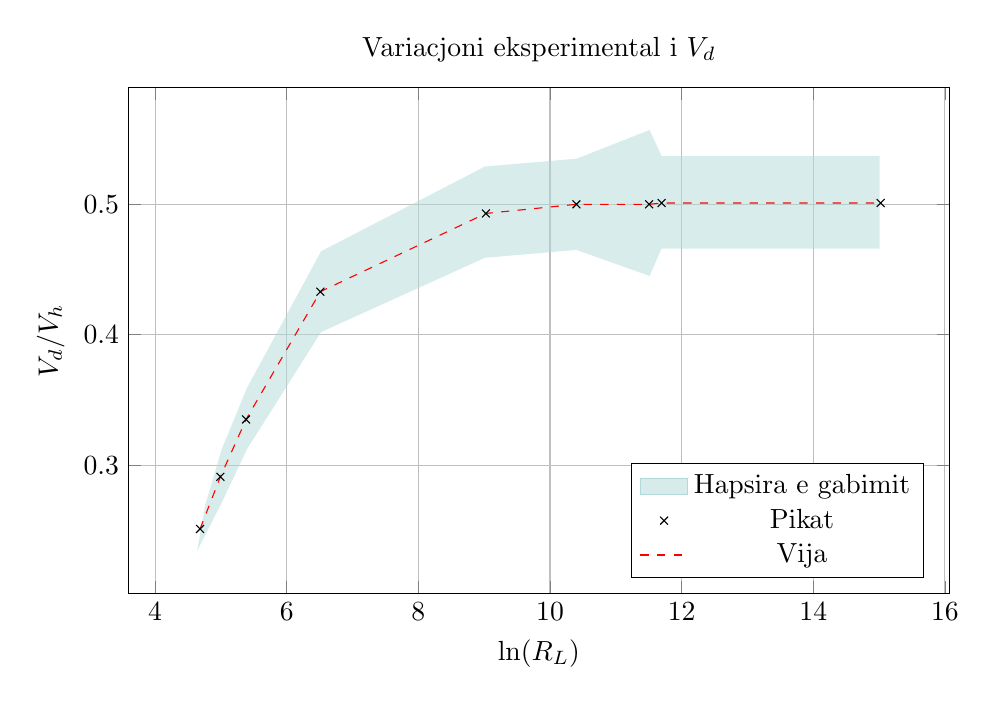
\begin{tikzpicture}
    \begin{axis}[
        xlabel={$\ln(R_L)$},
        ylabel={$V_d/V_h$},
        title={Variacjoni eksperimental i $V_d$ },
        grid=major,
        legend pos=south east,
        width=12cm,
        height=8cm
    ]
    
    %Lower bound
    \addplot[name path=lower, draw=none, forget plot] coordinates {
        (4.638, 0.234)
        (5.011, 0.271)
        (5.394, 0.312)
        (6.522, 0.402)
        (9.012, 0.459)
        (10.404, 0.465)
        (11.513, 0.445)
        (11.695, 0.466)
        (15.009, 0.466)
    };

    %Upper bound
    \addplot[name path=upper, draw=none, forget plot] coordinates {
        (4.760, 0.269)
        (5.011, 0.312)
        (5.394, 0.359)
        (6.522, 0.464)
        (9.012, 0.529)
        (10.404, 0.535)
        (11.513, 0.557)
        (11.695, 0.537)
        (15.009, 0.537)
    };

    % Filled area between bounds
    \addplot[teal!30, fill opacity=0.5] 
        fill between[of=lower and upper];
    \addlegendentry{Hapsira e gabimit}

    %Data points
    \addplot[only marks, black, mark=x] coordinates {
        (4.683, 0.251)
        (4.992, 0.291)
        (5.382, 0.335)
        (6.511, 0.433)
        (9.026, 0.493)
        (10.401, 0.5)
        (11.506, 0.5)
        (11.695, 0.501)
        (15.024, 0.501)
    };
    \addlegendentry{Pikat}

    %Dashed line
    \addplot[red, dashed] coordinates {
        (4.683, 0.251)
        (4.992, 0.291)
        (5.382, 0.335)
        (6.511, 0.433)
        (9.026, 0.493)
        (10.401, 0.5)
        (11.506, 0.5)
        (11.695, 0.501)
        (15.024, 0.501)
    };
    \addlegendentry{Vija}

    \end{axis}
\end{tikzpicture}

\end{document}